\documentclass[10pt,letterpaper]{article}

\usepackage[utf8]{inputenc}
\usepackage{amsmath}
\usepackage{amssymb}
\usepackage{graphicx}
\usepackage{enumitem}
\usepackage{gensymb}

\DeclareMathOperator{\arcsec}{arcsec}
\DeclareMathOperator{\arccot}{arccot}
\DeclareMathOperator{\arccsc}{arccsc}

\usepackage{multicol}
\setlength{\columnseprule}{1pt}
\def\columnseprulecolor{\color{black}}

\usepackage{pgfplots}
\usepgfplotslibrary{fillbetween}

\newcommand{\ihat}{\hat{\textbf{\i}}}
\newcommand{\jhat}{\hat{\textbf{\j}}}
\newcommand{\uhat}{\hat{\textbf{\u}}}

\usepackage[top=1in, bottom=1in, left=1in, right=1in]{geometry}


\begin{document}

\begin{titlepage}
    \centering

    {\scshape\LARGE Universidad Nacional Autónoma de México \par}

    \vspace{1cm}
    {\scshape\Large Facultad de Ciencias\par}
    \vspace{1.5cm}

    \begin{center}
        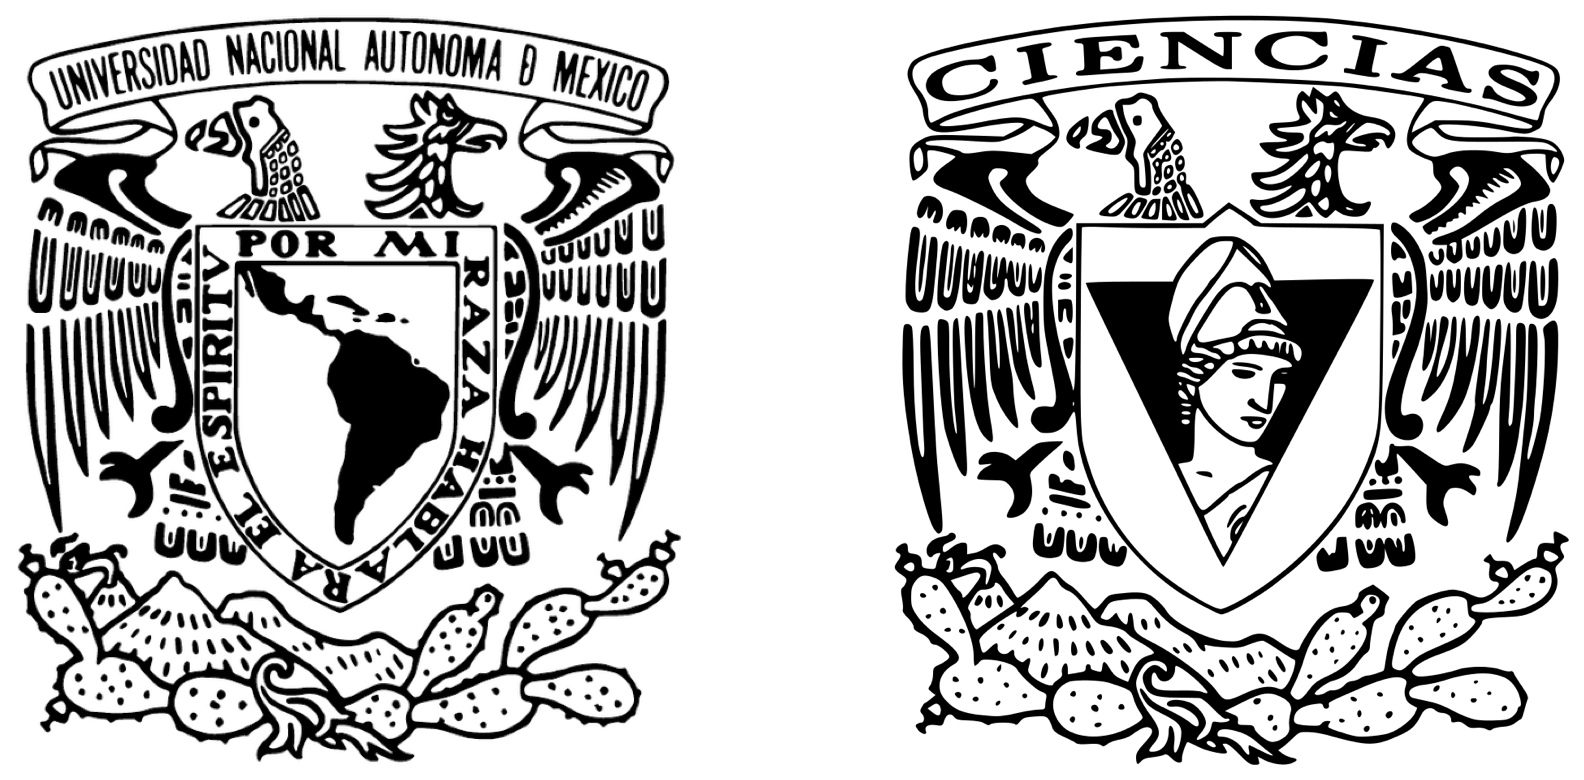
\includegraphics[scale=.1]{Images/logo.png}
    \end{center}

    \vspace{.8 cm}

    {\LARGE Examen 2: \par}
    {\huge\bfseries Sólidos de revolución \par}

    \vspace{0.5cm}
    \large{\itshape{Sebastián Alamina Ramírez}} \small{ - 318685496} \\ \vspace{0.3cm}

    \vfill

    \textbf{Matemáticas para las Ciencias Aplicadas II}
    \par
    \vspace{0.5cm}
    Fecha de entrega: \textbf{25 de Marzo de 2019}.
\end{titlepage}

\begin{enumerate}

% 1 ----------------------------------------------------------------------------------------------
\item Encuentra el volumen del sólido formado por la región encerrada por las curvas $y=e^{-x^2}$,
      $y=0$, $x=0$ y $x=1$ al rotar al rededor del eje $y$.

\begin{multicols}{2}

%Gráfica (1)
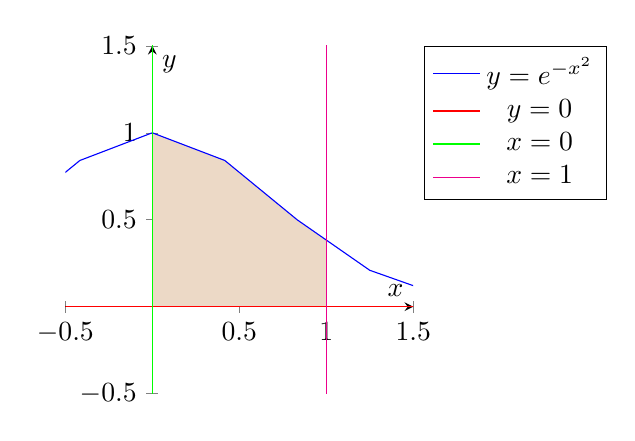
\begin{tikzpicture}
    \begin{axis}[xmin= -0.5, xmax= 1.5, ymin= -0.5, ymax= 1.5, width= 6cm, height= 6cm,
        xtick distance= 0.5, ytick distance = 0.5, xlabel=$x$, ylabel=$y$, axis lines=center,
        legend entries={$y=e^{-x^2}$, $y=0$, $x=0$, $x=1$},
        legend style={legend pos=outer north east} ]

        %\addplot[domain=x:x, mark]{};
        \addplot[name path=a, mark=none, blue]{ e^(-x^2) }; %y=e^{-x^2}
        \addplot[name path=b, mark=none, red](x,0); %y=0
        \addplot[mark=none, green](0,x); %x=0
        \addplot[mark=none, magenta](1,x); %x=1

        %Sombrear área
        \addplot fill between[ 
            of = a and b,
            soft clip = {domain = 0:1},
            %split, % calculate segments
            every even segment/.style = {brown!30},
            every odd segment/.style  = {brown!30}
        ];
    \end{axis}
\end{tikzpicture}

%Planteamiento (1)
\textbf{Planteamiento:}

\textit{Por discos...} \\
$r = x$
$$V = \int_{0}^{1} \pi x^2\ dy$$
Pero $x$ se dividiría en dos intervalos... Sea $\lambda$ la intersección entre $x=1$ y $y=-e^{x^2}$,
entonces el método por discos sería:
$$V = \int_{0}^{\lambda} \pi\ dy + \int_{\lambda}^{1} \pi( \sqrt{-\ln{y}} )^2\ dy $$

\textit{Por cilindros...} \\
$r = x$ \\
$h = e^{-x^2}$
$$V = \int_{0}^{1} 2 \pi x e^{-x^2}\ dx$$

%Solución (1)
\textbf{Solución:}

\textit{Por cilindros...}
$$V = \int_{0}^{1} 2 \pi x e^{-x^2}\ dx = 2\pi \int_{0}^{1} x e^{-x^2}\ dx$$ \\
Sea $u = -x^2$, ent. $du = -2x\ dx \implies dx = \frac{du}{-2x}$
$$V = 2\pi \int_{x=0}^{x=1} -\frac{x}{2x} e^u\ du = -\pi \int_{x=0}^{x=1} e^u\ du$$
$$= -\pi[e^u]_{x=0}^{x=1} = -\pi[e^{-x^2}]_{x=0}^{x=1} = -\pi[e^{-1}-e^0]$$
$$= -\pi[\frac{1}{e}-1] = \pi - \frac{\pi}{e}$$

\end{multicols}

% 2 ----------------------------------------------------------------------------------------------
\item Encuentra el volumen del sólido formado por la región encerrada por las curvas $y=x^2 +1$,
      $y=x+3$ al rotar alrededor del eje $y = -1$.

\begin{multicols}{2}

%Gráfica (2)
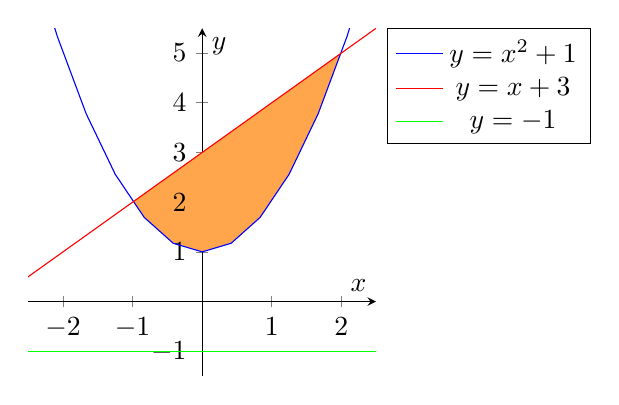
\begin{tikzpicture}
    \begin{axis}[xmin= -2.5, xmax= 2.5, ymin= -1.5, ymax= 5.5, width= 6cm, height= 6cm,
        xtick distance= 1, ytick distance = 1, xlabel=$x$, ylabel=$y$, axis lines=center,
        legend entries={$y=x^2 +1$, $y=x+3$, $y = -1$},
        legend style={legend pos=outer north east} ]

        %\addplot[domain=x:x, mark]{};
        \addplot[name path=a, mark=none, blue]{ x^(2) + 1 }; %y=x^2 +1
        \addplot[name path=b, mark=none, red]{ x+3 }; %y=x+3
        \addplot[mark=none, green](x,-1); %y = -1

        %Sombrear área
        \addplot fill between[ 
            of = a and b,
            soft clip = {domain = -1:2},
            split, % calculate segments
            every even segment/.style = {orange!70},
            every odd segment/.style  = {brown!30}
        ];
    \end{axis}
\end{tikzpicture}

%Planteamiento (2)
\textbf{Planteamiento:}

\textit{Por discos...} \\
$r_m = (x^2 + 1) + 1 = x^2 + 2$ \\
$r_M = (x + 3) + 1 = x + 4$
$$V = \int_{-1}^{2} \pi ( (x+4)^2 - (x^2 + 2)^2 ) \ dx$$

\textit{Por cilindros...} \\
$r = (x+3)+1 = x+4$ \\
$h = $Aquí se "complica", $\therefore$ se resuelve por discos...

%Solución (2)
\textbf{Solución:}

\textit{Por discos...}
$$V = \int_{-1}^{2} \pi ( (x+4)^2 - (x^2 + 2)^2 ) \ dx$$
$$= \pi \int_{-1}^{2} (x^2 + 8x + 16 - x^4 - 4x^2 -4) \ dx$$
$$= \pi \int_{-1}^{2} (-x^4 -3x^2 + 8x + 12)\ dx$$
$$= \pi [\frac{-x^5}{5} - x^3 + 4x^2 + 12x]_{-1}^{2}$$
$$= \pi [\frac{-32}{5} - 8 + 16 + 24 - \frac{1}{5} - 1 - 4  + 12]$$
$$= \pi [\frac{-33}{5}+39] = \pi [\frac{-33}{5} + \frac{195}{5}] = \frac{162}{5}\pi$$

\end{multicols}
\newpage

% 3 ----------------------------------------------------------------------------------------------
\item Encuentra el volumen del sólido generado al hacer rotar alrededor de la recta $y=2$ la región
      acotada por las curvas $y = \sec x$, $y = 0$, $0 \leq x \leq \pi/3$.

\begin{multicols}{2}

%Gráfica (3)
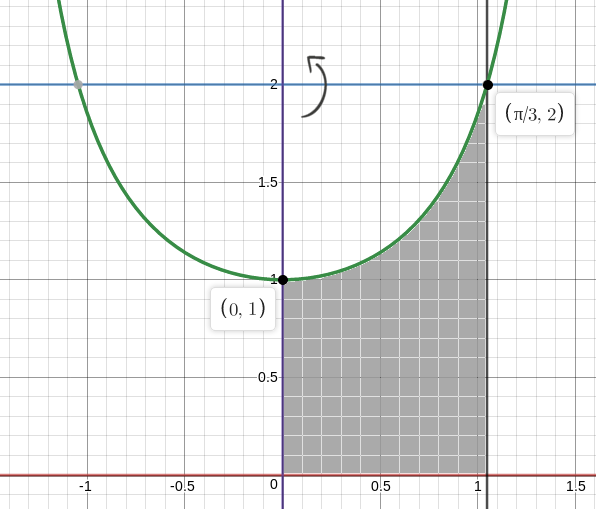
\includegraphics[width=5cm]{Images/grafica3.png}

%Planteamiento (3)
\textbf{Planteamiento:}

\textit{Por discos...} \\
$r_m = 2 - \sec x$ \\
$r_M = 2$
$$V = \int_{0}^{\pi/3} \pi ( (2)^2 - (2 - \sec x)^2 ) \ dx$$

\textit{Por cilindros...} \\
$r = (2-y)$ \\
$h = \pi/3$ con $0 \leq y \leq 1$ \\
y $h = \pi/3 - \arcsec(y)$ con $1 \leq y \leq 2$
$$V = \int_{0}^{1} 2\pi (2-y) (\pi/3)\ dy \rightarrow$$
$$+ \int_{1}^{2} 2\pi (2-y) ( \pi/3 - \arcsec(y) )\ dy$$

%Solución (3)
\textbf{Solución:}

\textit{Por discos...}
$$V = \int_{0}^{\pi/3} \pi ( (2)^2 - (2 - \sec x)^2 ) \ dx$$
$$= \pi \int_{0}^{\pi/3} (4 - 4 + 4\sec x - \sec^2 x)\ dx$$
$$= \pi \int_{0}^{\pi/3} (4\sec x - \sec^2 x)\ dx$$
$$= \pi \bigg[ 4 \int_{0}^{\pi/3} \sec x \ dx - \int_{0}^{\pi/3} \sec^2 x\ dx \bigg]$$
$$= \pi \bigg[ 4 \Big[ \ln{(\tan x+\sec x)} \Big]_{0}^{\pi/3} - \Big[ \tan x \Big]_{0}^{\pi/3} \bigg] $$
$$= \pi \bigg[ 4 \Big[ \ln{(\tan \frac{\pi}{3}+\sec \frac{\pi}{3})} - \ln{(\tan 0+\sec 0)} \Big] \rightarrow$$
$$- \Big[ \tan \frac{\pi}{3} - \tan 0 \Big] \bigg] $$
$$= \pi \bigg[ 4 \Big[ \ln{(\sqrt{3}+2)} - \ln{(0+1)} \Big] - \Big[ \sqrt{3} - 0 \Big] \bigg]$$
$$= \pi \bigg[ 4 \Big[ \ln{(\sqrt{3}+2)} - 0 \Big] - \sqrt{3} \bigg]$$
$$= \pi \bigg( 4 \ln{(\sqrt{3}+2)} - \sqrt{3} \bigg) \approx 11.1079...$$

\end{multicols}


% 4 ----------------------------------------------------------------------------------------------
\item Halla el volumen del sólido de revolución generado al hacer rotar la región acotada por las
      curvas $y = x^2$, $y = 4x - x^2$ , en torno a la recta $x = 2$.

\begin{multicols}{2}

%Gráfica (4)
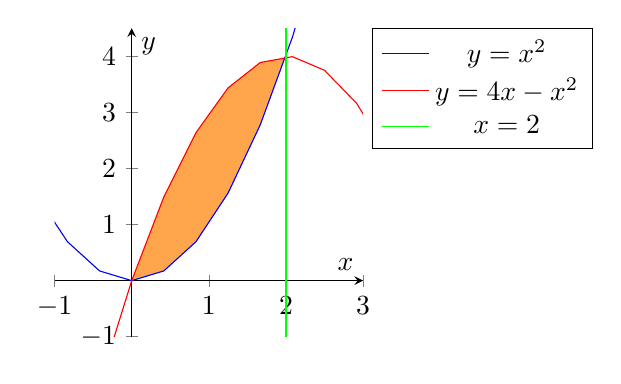
\begin{tikzpicture}
    \begin{axis}[xmin= -1, xmax= 3, ymin= -1, ymax= 4.5, width= 5.5cm, height= 5.5cm,
        xtick distance= 1, ytick distance = 1, xlabel=$x$, ylabel=$y$, axis lines=center,
        legend entries={$y=x^2$, $y=4x - x^2$, $x = 2$},
        legend style={legend pos=outer north east} ]

        %\addplot[domain=x:x, mark]{};
        \addplot[name path=a, mark=none, blue]{ x^2 }; %y=x^2
        \addplot[name path=b, mark=none, red]{ 4*x - x^2 }; %y=4x - x^2
        \addplot[mark=none, green](2,x); %x = 2

        %Sombrear área
        \addplot fill between[ 
            of = a and b,
            soft clip = {domain = 0:2},
            split, % calculate segments
            every even segment/.style = {orange!70},
            every odd segment/.style  = {brown!30}
        ];
    \end{axis}
\end{tikzpicture}

%Planteamiento (4)
\textbf{Planteamiento:}

\textit{Por discos...} \\
$r_m = 2-\sqrt{y}$ \\
$r_M = 2-(-\sqrt{4-y} + 2) = \sqrt{4-y}$
$$V = \int_{0}^{4} \pi ( (\sqrt{4-y})^2 - (2-\sqrt{y})^2 ) \ dy$$ \\

\textit{Por cilindros...} \\
$r = 2-x$ \\
$h = (4x-x^2)-(x^2) = -2x^2 + 4x$
$$V = \int_{0}^{2} 2\pi (2-x)(-2x^2+4x)\ dx$$

%Solución (4)
\textbf{Solución:}

\textit{Por cilindros...}
$$V = 2\pi \int_{0}^{2} (2-x)(-2x^2+4x)\ dx$$
$$= 2\pi \int_{0}^{2} (2x^3 - 8x^2 + 8x)\ dx$$
$$= 2\pi \bigg[ \frac{x^4}{2} - \frac{8x^3}{3} + 4x^2 \bigg]_{0}^{2}
= 2\pi \bigg[ \frac{16}{2} - \frac{64}{3} + 16 \bigg]$$
$$= 2\pi \bigg[ -\frac{80}{6} + 16 \bigg] = 2\pi \Big( \frac{16}{6} \Big)
= \frac{16\pi}{3}$$

\end{multicols}

\newpage

% 5 ----------------------------------------------------------------------------------------------
\item Determina el volumen de la región encerrada entre las curvas $y = 1 + x^2$ y $y = 0$ al rotar
      alrededor del eje $x$ cuando $0 \leq x \leq 2$.

\begin{multicols}{2}

%Gráfica (5)
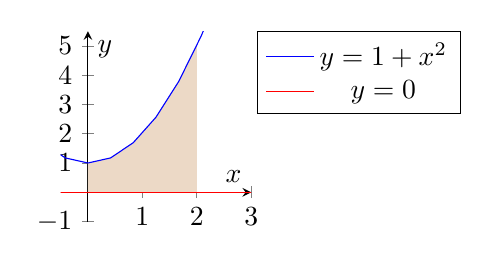
\begin{tikzpicture}
    \begin{axis}[xmin= -0.5, xmax= 3, ymin= -1, ymax= 5.5, width= 4cm, height= 4cm,
        xtick distance= 1, ytick distance = 1, xlabel=$x$, ylabel=$y$, axis lines=center,
        legend entries={$y=1+x^2$, $y=0$},
        legend style={legend pos=outer north east} ]

        %\addplot[domain=x:x, mark]{};
        \addplot[name path=a, mark=none, blue]{ 1 + x^2 }; %y=1+x^2
        \addplot[name path=b, mark=none, red](x,0); %y=0

        %Sombrear área
        \addplot fill between[ 
            of = a and b,
            soft clip = {domain = 0:2},
            %split, % calculate segments
            every even segment/.style = {brown!30},
            every odd segment/.style  = {brown!30}
        ];
    \end{axis}
\end{tikzpicture}

%Planteamiento (5)
\textbf{Planteamiento:}

\textit{Por discos...} \\
$r = 1+x^2$ \\
$$V = \int_{0}^{2} \pi (1+x^2)^2\ dx$$
\textit{Por cilindros...} \\
$r = y$ \\
$h = 2$ con $0 \leq y \leq 1$ \\
$h = 2 - \sqrt{y-1}$ con $1 \leq y \leq 5$
$$V = \int_{0}^{1} 2\pi y (2)\ dy + \int_{1}^{5} 2\pi y (2-\sqrt{y-1})\ dy$$

%Solución (5)
\textbf{Solución:}

\textit{Por discos...}
$$V = \int_{0}^{2} \pi (1+x^2)^2\ dx$$
$$= \pi \int_{0}^{2} (1 + 2x^2 + x^4)\ dx$$
$$= \pi \bigg[ x + \frac{2x^3}{3} + \frac{x^5}{5} \bigg]_{0}^{2}$$
$$= \pi \bigg[ 2 + \frac{16}{3} + \frac{32}{5} - 0 - 0 - 0 \bigg]$$
$$= \pi \bigg[ 2 + \frac{176}{15} \bigg]$$
$$= \frac{206\pi}{15}$$


\end{multicols}

% 6 ----------------------------------------------------------------------------------------------
\item Determina el volumen de la región encerrada por la función $x = \sqrt{\sin y}$ con
      $0 \leq y \leq \pi$ y $x = 0$ si rota en $y = 4$.

\begin{multicols}{2}

%Gráfica (6)
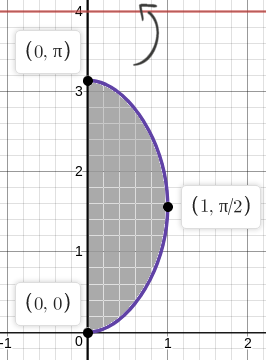
\includegraphics[height=4cm]{Images/grafica5.png}

%Planteamiento (6)
\textbf{Planteamiento:}

\textit{Por discos...} \\
$r_m = (4-\pi) + \arcsin{x^2}$ \\
$r_M = 4 - \arcsin{x^2}$
$$V = \int_{0}^{1} \pi ( (4 - \arcsin{x^2})^2 - ((4-\pi) + \arcsin{x^2})^2 ) \ dx$$

\textit{Por cilindros...} \\
$r = 4-y$ \\
$h = \sqrt{\sin y}$
$$V = \int_{0}^{\pi} 2\pi (4-y) (\sqrt{\sin y})\ dy$$

%Solución (6)
\textbf{Solución:}\\
Estas integrales no tienen una solución concreta. Sin embargo, ambas arrojan como resultado un
aproximado de 36.574756682... al utilizar "integración numérica".

\end{multicols}

\newpage

% 7 ----------------------------------------------------------------------------------------------
\item Determinar la superficie del sólido de revolución generado al rotar en el eje $y$ la región
      definida por $y = x^3$ con $0 \leq x \leq 1$.

\begin{multicols}{2}

%Gráfica (7)
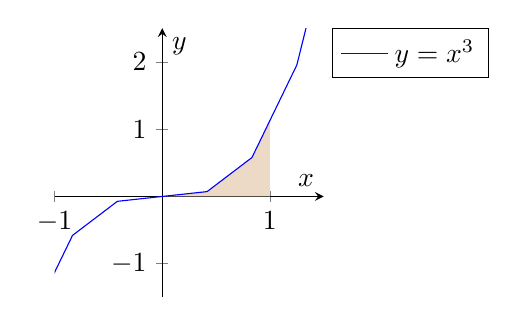
\begin{tikzpicture}
    \begin{axis}[xmin= -1, xmax= 1.5, ymin= -1.5, ymax= 2.5, width= 5cm, height= 5cm,
        xtick distance= 1, ytick distance = 1, xlabel=$x$, ylabel=$y$, axis lines=center,
        legend entries={$y=x^3$},
        legend style={legend pos=outer north east} ]

        %\addplot[domain=x:x, mark]{};
        \addplot[name path=a, mark=none, blue]{ x^3 }; % y=x^3
        \addplot[name path=b, draw=none](x,0);

        Sombrear área
        \addplot fill between[ 
            of = a and b,
            soft clip = {domain = 0:1},
        %    %split, % calculate segments
            every even segment/.style = {brown!30},
            every odd segment/.style  = {brown!30}
        ];
    \end{axis}
\end{tikzpicture}

%Planteamiento (7)
\textbf{Planteamiento:}

\textit{Con dx...} \\
$r = x$
$$S = \int_{0}^{1} 2\pi x \sqrt{1+ (3x^2)^2 }\ dx$$

\textit{Con dy...} \\
$r = x = \sqrt[3]{y}$
$$S = \int_{0}^{1} 2\pi (\sqrt[3]{y}) \sqrt{1+ (\frac{y^{-2/3}}{3})^2 }\ dx$$

%Solución (7)
\textbf{Solución:}

\textit{Con dx...}
$$S = 2\pi \int_{0}^{1} x \sqrt{1+ 9x^4 }\ dx$$
Sea $u=x^2 \implies du = 2x\ dx$\\
$\implies dx = \frac{du}{2x}$
$$S = 2\pi \int_{0}^{1} \frac{1}{2x} x \sqrt{1+ 9u^2 }\ du$$
$$= \pi \int_{0}^{1} \sqrt{1+ 9u^2 }\ du$$
Sea $\alpha$ el ángulo diferente de $90\degree$ en un ángulo rectángulo tal que:\\
$H = \sqrt{1+9u^2}$, $CO = 3u$ y $CA = 1$.\\
$\tan \alpha = \frac{CO}{CA} = 3u \implies u = \frac{\tan \alpha}{3}$\\
Y $du = \frac{\sec^2\alpha}{3}\ d\alpha$
$$S = \pi \int_{u=0}^{u=1} \sqrt{1+ 9(\frac{\tan \alpha}{3})^2 }\ \frac{\sec^2\alpha}{3}\ d\alpha$$
$$= \frac{\pi}{3} \int_{u=0}^{u=1} \sqrt{1+ \tan^2 \alpha }\ \sec^2\alpha\ d\alpha$$
$$= \frac{\pi}{3} \int_{u=0}^{u=1} \sqrt{\sec^2\alpha}\ \sec^2\alpha\ d\alpha$$
$$= \frac{\pi}{3} \int_{u=0}^{u=1} \sec^3 \alpha\ d\alpha$$
Tenemos que $\int \sec^3x\ dx = \frac{\sec x \tan x}{2} + \frac{1}{2} \int \sec x\ dx$
$$S = \frac{\pi}{3} \bigg(
\Big[ \frac{\sec \alpha \tan \alpha}{2} \Big]_{u=0}^{u=1}
+ \frac{1}{2} \int_{u=0}^{u=1} \sec \alpha\ d\alpha \bigg)$$
$$= \frac{\pi}{3} \bigg(
\Big[ \frac{\sec \alpha \tan \alpha}{2} \Big]_{u=0}^{u=1}
+ \frac{1}{2} \Big[ \ln{(\tan \alpha+\sec \alpha)} \Big]_{u=0}^{u=1} \bigg)$$
Pero $\tan\alpha = 3u$ y $\sec\alpha = \sqrt{1+9u^2}$
$$S = \frac{\pi}{3} \bigg(
\Big[ \frac{\sqrt{1+9u^2}\ 3u}{2} \Big]_{0}^{1}
+ \frac{1}{2} \Big[ \ln{(3u+\sqrt{1+9u^2})} \Big]_{0}^{1} \bigg)$$
$$= \frac{\pi}{3} \bigg(
\Big[ 3\frac{ \sqrt{10} }{2} - 0 \Big]
+ \frac{1}{2} \Big[ \ln{(3+\sqrt{10})} - 0 \Big] \bigg)$$
$$= \pi \bigg( \frac{ \sqrt{10} }{2}
+ \frac{1}{6} \Big[ \ln{(3+\sqrt{10})} \Big] \bigg)$$
$$= \pi \bigg( \frac{ 3\sqrt{10} + \ln{ (3+\sqrt{10}) }}{6} \bigg)
\approx 5.9194304... $$

\end{multicols}

\end{enumerate}

\end{document}